\documentclass[11pt,a4paper]{article}

\usepackage[top=20mm,bottom=26mm,left=20mm,right=20mm,headheight=15pt,footskip=12mm]{geometry}

\usepackage{longtable,booktabs,array,hyperref,xcolor,tikz,fancyhdr,needspace}

\usepackage{fontspec,xeCJK}

\setmainfont[Ligatures=TeXOff]{Times New Roman}

\setsansfont[Ligatures=TeXOff]{Times New Roman}

\setmonofont[Ligatures=TeXOff,WordSpace={1,1,1}]{Times New Roman}

\setCJKmainfont{Noto Serif CJK SC}

\setCJKsansfont{Noto Serif CJK SC}

\setCJKmonofont{Noto Serif CJK SC}

\newfontfamily\vulcanmathsymbols{Noto Serif CJK SC}

\XeTeXgenerateactualtext=1

\definecolor{vulcan}{HTML}{BB3E23}

\definecolor{vulcanblue}{HTML}{1B4F72}

\renewcommand{\thesection}{\Roman{section}}

\renewcommand{\thesubsection}{\Alph{subsection}}

\pgfdeclarelayer{connections}\pgfdeclarelayer{edge labels}\pgfsetlayers{connections,main,edge labels}

\hypersetup{hidelinks}

\newcolumntype{L}[1]{>{\raggedright\arraybackslash\hspace{0pt}}p{#1}}

\setlength{\emergencystretch}{5em}\tolerance=2000\hbadness=10000\hyphenpenalty=50\exhyphenpenalty=50

\setlength{\parindent}{0pt}\setlength{\parskip}{5pt}

\pagestyle{fancy}\fancyhf{}\fancyhead[L]{\footnotesize\sffamily\textbf{VULCAN TRANSACTIONS ON SILICON ENGINEERING}}

\fancyhead[R]{\footnotesize\sffamily RTL Microarchitecture \& Silicon Signoff}\fancyfoot[C]{\footnotesize\sffamily Page \thepage}

\begin{document}

{\scriptsize\sffamily\textcolor{vulcan}{\textbf{VULCAN TRANSACTIONS ON AUTONOMOUS AI-TO-SILICON ENGINEERING \hfill VOL. 2026 \textperiodcentered{} ARCHITECTURAL SIGNOFF PAPER}}\par}

\vspace{1pt}\textcolor{vulcan}{\rule{\textwidth}{1.2pt}}\vspace{4pt}

\begin{center}

{\sffamily\LARGE\bfseries BILLET-F1 Programmable-Coefficient FIR IP\par}\vspace{3pt}

{\small\sffamily\textbf{Sufeng Guo (\allowbreak{}sufeng\_\allowbreak{}guo@smail.nju.edu.cn)\allowbreak{}} \textperiodcentered{} Microsoft Research Asia \textperiodcentered{} Technical Design and Verification Report\par}\vspace{1pt}

{\scriptsize\sffamily\textcolor{black!75}{Silicon Platform: Intel Arria 10 GX (\texttt{10AX115N3F40E2SG}) PCIe Gen3x8 \textperiodcentered{} Toolchain: Icarus Verilog 12.0 / Yosys 0.33 / Quartus Prime 17.1 STA \textperiodcentered{} 24 October 2026 (\allowbreak{}2026-10-24 20:14 UTC+\allowbreak{}8 Beijing Time)\allowbreak{}}\par}

\end{center}\vspace{2pt}

\renewcommand{\abstractname}{\textcolor{vulcanblue}{Abstract}}\begin{abstract}\noindent BILLET-F1 is a synthesizable,\allowbreak{} single-clock streaming FIR filter for signed 16-bit Q1.15 samples and programmable coefficients. It supports 1,\allowbreak{} 8,\allowbreak{} 16,\allowbreak{} 32 and 64 taps,\allowbreak{} defaulting to 32. Full-width accumulation,\allowbreak{} round-to-nearest ties-to-even,\allowbreak{} output saturation and double-buffered coefficient commits provide deterministic numerical behavior without mixing coefficient generations. Independent Icarus simulation completed all 15 tap-count/\allowbreak{}seed combinations and checked 106,\allowbreak{}971 completed results with zero bit mismatches. Measured output-availability latency is T cycles and sustained always-ready initiation interval is T+\allowbreak{}1 cycles. Three separately executed RTL mutants produced numerical mismatches. Yosys structural and synthesis checks passed for all five legal configurations,\allowbreak{} and fresh-directory partial reproduction independently regenerated behavioral,\allowbreak{} defect and default-configuration synthesis results. These conclusions concern functional RTL and generic synthesis,\allowbreak{} not physical implementation.\par\vspace{2pt}{\scriptsize\textbf{\textcolor{vulcanblue}{Index Terms---}}Autonomous RTL Generation, SystemVerilog, Intel Arria 10 GX FPGA, TimeQuest 100~MHz+ Timing Closure, PCIe Gen3x8 Hardware-in-the-Loop (HIL), Bit-Exact Fixed-Point Verification.}\end{abstract}\vspace{2pt}

\needspace{5\baselineskip}\section{Architecture and design rationale}

The architecture shares one signed 16-by-16 multiplier across T sequential multiply-accumulate cycles. Sample history shifts only on input acceptance; computations do not overlap. Two coefficient banks separate active filtering from staging writes,\allowbreak{} while a completeness bitmap prevents partial-bank activation. A single registered output slot provides backpressure retention. This organization favors simple resource sharing and explicit ownership over one-sample-per-cycle throughput. The final product-plus-accumulator sum passes through combinational rounding and saturation before being registered on the final MAC edge,\allowbreak{} avoiding an additional output stage. The four source modules and literal child instances are preserved under the top-level g\_\allowbreak{}supported generate branch. [\allowbreak{}E002,\allowbreak{} E004-E007]\allowbreak{}

\begin{center}\begin{minipage}{\textwidth}\centering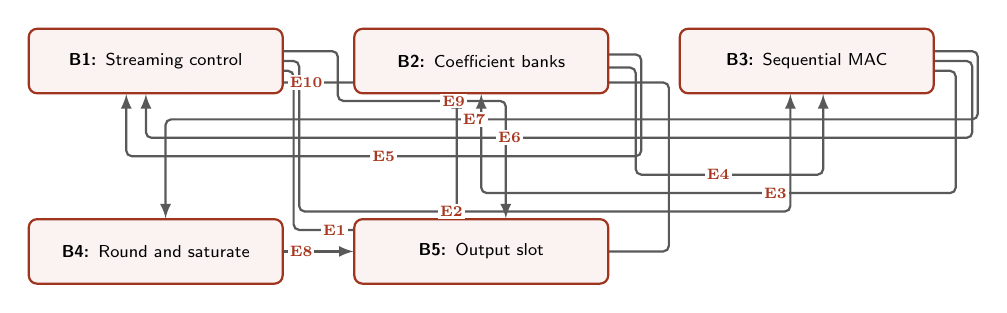
\begin{tikzpicture}[scale=0.78,transform shape,every node/.style={font=\footnotesize\sffamily},>=latex]

\node[draw=vulcan!85!black,thick,rounded corners=3pt,fill=vulcan!6,text width=3.9cm,minimum height=1.05cm,align=center] (b0) at (0.0,0.0) {\textbf{B1:} Streaming control};

\node[draw=vulcan!85!black,thick,rounded corners=3pt,fill=vulcan!6,text width=3.9cm,minimum height=1.05cm,align=center] (b1) at (5.3,0.0) {\textbf{B2:} Coefficient banks};

\node[draw=vulcan!85!black,thick,rounded corners=3pt,fill=vulcan!6,text width=3.9cm,minimum height=1.05cm,align=center] (b2) at (10.6,0.0) {\textbf{B3:} Sequential MAC};

\node[draw=vulcan!85!black,thick,rounded corners=3pt,fill=vulcan!6,text width=3.9cm,minimum height=1.05cm,align=center] (b3) at (0.0,-3.1) {\textbf{B4:} Round and saturate};

\node[draw=vulcan!85!black,thick,rounded corners=3pt,fill=vulcan!6,text width=3.9cm,minimum height=1.05cm,align=center] (b4) at (5.3,-3.1) {\textbf{B5:} Output slot};

\begin{pgfonlayer}{connections}

\draw[->,thick,black!65,rounded corners=2pt] ([yshift=-0.160cm]b0.east) -- (2.245,-0.160) -- (2.245,-2.750) -- coordinate[pos=0.25] (e0) (4.900,-2.750) -- ([xshift=-0.400cm]b1.south);

\draw[->,thick,black!65,rounded corners=2pt] ([yshift=0.000cm]b0.east) -- (2.335,0.000) -- (2.335,-2.450) -- coordinate[pos=0.31] (e1) (10.333,-2.450) -- ([xshift=-0.267cm]b2.south);

\draw[->,thick,black!65,rounded corners=2pt] ([yshift=-0.160cm]b2.east) -- (13.025,-0.160) -- (13.025,-2.150) -- coordinate[pos=0.38] (e2) (5.300,-2.150) -- ([xshift=0.000cm]b1.south);

\draw[->,thick,black!65,rounded corners=2pt] ([yshift=-0.107cm]b1.east) -- (7.815,-0.107) -- (7.815,-1.850) -- coordinate[pos=0.44] (e3) (10.867,-1.850) -- ([xshift=0.267cm]b2.south);

\draw[->,thick,black!65,rounded corners=2pt] ([yshift=0.107cm]b1.east) -- (7.905,0.107) -- (7.905,-1.550) -- coordinate[pos=0.50] (e4) (-0.480,-1.550) -- ([xshift=-0.480cm]b0.south);

\draw[->,thick,black!65,rounded corners=2pt] ([yshift=0.000cm]b2.east) -- (13.295,0.000) -- (13.295,-1.250) -- coordinate[pos=0.56] (e5) (-0.160,-1.250) -- ([xshift=-0.160cm]b0.south);

\draw[->,thick,black!65,rounded corners=2pt] ([yshift=0.160cm]b2.east) -- (13.385,0.160) -- (13.385,-0.950) -- coordinate[pos=0.62] (e6) (0.160,-0.950) -- ([xshift=0.160cm]b3.north);

\draw[->,thick,black!65] ([yshift=0.000cm]b3.east) -- coordinate[pos=0.25] (e7) ([yshift=0.000cm]b4.west);

\draw[->,thick,black!65,rounded corners=2pt] ([yshift=0.160cm]b0.east) -- (2.965,0.160) -- (2.965,-0.650) -- coordinate[pos=0.69] (e8) (5.700,-0.650) -- ([xshift=0.400cm]b4.north);

\draw[->,thick,black!65,rounded corners=2pt] ([yshift=0.000cm]b4.east) -- (8.355,-3.100) -- (8.355,-0.350) -- coordinate[pos=0.75] (e9) (0.480,-0.350) -- ([xshift=0.480cm]b0.south);

\end{pgfonlayer}

\begin{pgfonlayer}{edge labels}

\node[fill=white,inner sep=1pt,font=\scriptsize\bfseries,text=vulcan!90!black] at (e0) {E1};

\node[fill=white,inner sep=1pt,font=\scriptsize\bfseries,text=vulcan!90!black] at (e1) {E2};

\node[fill=white,inner sep=1pt,font=\scriptsize\bfseries,text=vulcan!90!black] at (e2) {E3};

\node[fill=white,inner sep=1pt,font=\scriptsize\bfseries,text=vulcan!90!black] at (e3) {E4};

\node[fill=white,inner sep=1pt,font=\scriptsize\bfseries,text=vulcan!90!black] at (e4) {E5};

\node[fill=white,inner sep=1pt,font=\scriptsize\bfseries,text=vulcan!90!black] at (e5) {E6};

\node[fill=white,inner sep=1pt,font=\scriptsize\bfseries,text=vulcan!90!black] at (e6) {E7};

\node[fill=white,inner sep=1pt,font=\scriptsize\bfseries,text=vulcan!90!black] at (e7) {E8};

\node[fill=white,inner sep=1pt,font=\scriptsize\bfseries,text=vulcan!90!black] at (e8) {E9};

\node[fill=white,inner sep=1pt,font=\scriptsize\bfseries,text=vulcan!90!black] at (e9) {E10};

\end{pgfonlayer}

\end{tikzpicture}\par\vspace{3pt}

{\small\textbf{Figure 1:} Top-level microarchitectural functional block map and directed inter-module bus topology.}\end{minipage}\end{center}

{\small\renewcommand{\arraystretch}{1.18}\begin{longtable}{@{}L{0.24\textwidth}|L{0.7\textwidth}@{}}\toprule

\textbf{Block} & \textbf{Responsibility}\\\midrule\endhead

B1: Streaming control & billet\_\allowbreak{}f1\_\allowbreak{}top arbitrates input,\allowbreak{} configuration and commit handshakes. It starts computations only when idle and output capacity is available,\allowbreak{} and permits commits only after computation and output drainage.\\[2pt]\hline

B2: Coefficient banks & billet\_\allowbreak{}f1\_\allowbreak{}coeff\_\allowbreak{}bank,\allowbreak{} instantiated as u\_\allowbreak{}coeff\_\allowbreak{}bank,\allowbreak{} owns two T-by-16 coefficient arrays,\allowbreak{} active-bank selection and the staging-written bitmap. It supplies the selected active coefficient asynchronously.\\[2pt]\hline

B3: Sequential MAC & billet\_\allowbreak{}f1\_\allowbreak{}mac,\allowbreak{} instantiated as u\_\allowbreak{}mac,\allowbreak{} owns shifted sample history,\allowbreak{} tap sequencing,\allowbreak{} busy state and full-width accumulation. Tap zero addresses the newest accepted sample.\\[2pt]\hline

B4: Round and saturate & billet\_\allowbreak{}f1\_\allowbreak{}round\_\allowbreak{}sat,\allowbreak{} instantiated as u\_\allowbreak{}round\_\allowbreak{}sat,\allowbreak{} implements signed ties-to-even division by 32768 followed by signed 16-bit saturation. It contains no state.\\[2pt]\hline

B5: Output slot & Registers within billet\_\allowbreak{}f1\_\allowbreak{}top retain the completed result and valid flag until transfer or reset. Invalid output data is explicitly zero.\\[2pt]\hline

\bottomrule\end{longtable}}

{\small\renewcommand{\arraystretch}{1.18}\begin{longtable}{@{}L{0.24\textwidth}|L{0.7\textwidth}@{}}\toprule

\textbf{Directed relationship} & \textbf{Meaning}\\\midrule\endhead

E1: B1 to B2 & Accepted staging writes and atomic commit\\[2pt]\hline

E2: B1 to B3 & Accepted sample and start pulse\\[2pt]\hline

E3: B3 to B2 & Active coefficient read address\\[2pt]\hline

E4: B2 to B3 & Signed active coefficient\\[2pt]\hline

E5: B2 to B1 & Staging completeness\\[2pt]\hline

E6: B3 to B1 & Busy and final-cycle status\\[2pt]\hline

E7: B3 to B4 & Full-width final sum\\[2pt]\hline

E8: B4 to B5 & Rounded and saturated result\\[2pt]\hline

E9: B1 to B5 & Completion capture and retirement control\\[2pt]\hline

E10: B5 to B1 & Pending-output occupancy\\[2pt]\hline

\bottomrule\end{longtable}}

\needspace{9\baselineskip}\section{Interfaces and configuration}

{\small\renewcommand{\arraystretch}{1.18}\begin{longtable}{@{}L{0.21\textwidth}|L{0.12\textwidth}|L{0.12\textwidth}|L{0.45\textwidth}@{}}\toprule

\textbf{Signal /\allowbreak{} group} & \textbf{Direction} & \textbf{Width} & \textbf{Contract}\\\midrule\endhead

clk,\allowbreak{} rst\_\allowbreak{}n & Input & 1 bit each & Single rising-edge clock and asynchronous active-low reset. Reset clears all state and forces every public output,\allowbreak{} including ready signals and m\_\allowbreak{}data,\allowbreak{} to zero.\\[2pt]\hline

s\_\allowbreak{}data; s\_\allowbreak{}valid /\allowbreak{} s\_\allowbreak{}ready & Input data and valid /\allowbreak{} output ready & Signed 16-bit data; 1-bit controls & A sample transfers when s\_\allowbreak{}valid \&\& s\_\allowbreak{}ready immediately before a rising edge. The producer holds valid and data while stalled. s\_\allowbreak{}ready =\allowbreak{} rst\_\allowbreak{}n \&\& !busy \&\& (\allowbreak{}!m\_\allowbreak{}valid || m\_\allowbreak{}ready)\allowbreak{} \&\& !commit\_\allowbreak{}valid.\\[2pt]\hline

m\_\allowbreak{}data; m\_\allowbreak{}valid /\allowbreak{} m\_\allowbreak{}ready & Output data and valid /\allowbreak{} input ready & Signed 16-bit data; 1-bit controls & A result transfers on m\_\allowbreak{}valid \&\& m\_\allowbreak{}ready. Valid stalled data remains bit-stable; m\_\allowbreak{}data is zero whenever m\_\allowbreak{}valid is zero. Output retirement may coincide with acceptance of the next sample.\\[2pt]\hline

cfg\_\allowbreak{}addr,\allowbreak{} cfg\_\allowbreak{}data; cfg\_\allowbreak{}valid /\allowbreak{} cfg\_\allowbreak{}ready & Input address,\allowbreak{} data and valid /\allowbreak{} output ready & ADDR\_\allowbreak{}W-bit unsigned address; signed 16-bit coefficient; 1-bit controls & Accepted writes modify only the inactive staging bank. Repeated writes are legal and the latest value wins. cfg\_\allowbreak{}ready =\allowbreak{} rst\_\allowbreak{}n \&\& !commit\_\allowbreak{}valid \&\& (\allowbreak{}cfg\_\allowbreak{}addr < TAP\_\allowbreak{}COUNT)\allowbreak{}. At T=\allowbreak{}1,\allowbreak{} address 1 is invalid and never accepted.\\[2pt]\hline

commit\_\allowbreak{}valid /\allowbreak{} commit\_\allowbreak{}ready & Input request /\allowbreak{} output ready & 1 bit each & A handshake atomically swaps bank roles. commit\_\allowbreak{}ready =\allowbreak{} rst\_\allowbreak{}n \&\& staging\_\allowbreak{}complete \&\& !busy \&\& !m\_\allowbreak{}valid. Any asserted request blocks sample acceptance and configuration writes,\allowbreak{} including when the requested commit is not yet ready.\\[2pt]\hline

\bottomrule\end{longtable}}

{\small\renewcommand{\arraystretch}{1.18}\begin{longtable}{@{}L{0.22\textwidth}|L{0.21\textwidth}|L{0.49\textwidth}@{}}\toprule

\textbf{Parameter} & \textbf{Default} & \textbf{Meaning /\allowbreak{} supported values}\\\midrule\endhead

TAP\_\allowbreak{}COUNT & 32 & Only 1,\allowbreak{} 8,\allowbreak{} 16,\allowbreak{} 32 and 64 are legal. Unsupported values produce an explicit PARAMETER ERROR diagnostic rather than selecting a substitute datapath.\\[2pt]\hline

ADDR\_\allowbreak{}W & 5 at TAP\_\allowbreak{}COUNT=\allowbreak{}32 & Derived local parameter max(\allowbreak{}1,\allowbreak{} ceil(\allowbreak{}log2(\allowbreak{}TAP\_\allowbreak{}COUNT)\allowbreak{})\allowbreak{})\allowbreak{}; not independently configurable.\\[2pt]\hline

ACC\_\allowbreak{}W & 37 at TAP\_\allowbreak{}COUNT=\allowbreak{}32 & Derived local parameter 32+\allowbreak{}ceil(\allowbreak{}log2(\allowbreak{}TAP\_\allowbreak{}COUNT)\allowbreak{})\allowbreak{}; widths are 32,\allowbreak{} 35,\allowbreak{} 36,\allowbreak{} 37 and 38 bits for the supported tap counts.\\[2pt]\hline

Numerical formats & Signed 16-bit Q1.15 & Samples,\allowbreak{} coefficients and outputs have fixed widths. Products are signed 32 bits; intermediate sums retain full accumulator precision.\\[2pt]\hline

\bottomrule\end{longtable}}

\needspace{16\baselineskip}\section{Behavior and corner cases}

\subsection{Convolution and numerical transformation}

For accepted sample n,\allowbreak{} A[\allowbreak{}n]\allowbreak{} =\allowbreak{} sum over k=\allowbreak{}0 through T-1 of signed(\allowbreak{}x[\allowbreak{}n-k]\allowbreak{})\allowbreak{}*\allowbreak{}signed(\allowbreak{}c[\allowbreak{}k]\allowbreak{})\allowbreak{},\allowbreak{} with absent history zero. Set q=\allowbreak{}floor(\allowbreak{}A/\allowbreak{}32768)\allowbreak{} and r=\allowbreak{}A-32768*\allowbreak{}q. Increment q if r>16384,\allowbreak{} or if r=\allowbreak{}16384 and q is odd; then clamp to [\allowbreak{}-32768,\allowbreak{}32767]\allowbreak{}. This handles both signs symmetrically: accumulators -16384 and -49152 round to 0 and -2. An extended quotient prevents rounding overflow. In normalized units X=\allowbreak{}x/\allowbreak{}32768 and C=\allowbreak{}c/\allowbreak{}32768,\allowbreak{} the unclipped convolution is A/\allowbreak{}2\textasciicircum{}30. [\allowbreak{}E003,\allowbreak{} E005,\allowbreak{} E006]\allowbreak{}

\needspace{10\baselineskip}\subsection{Exact cycle schedule}

A handshake at E0 inserts the sample and starts computation. Edges E1 through E\_\allowbreak{}T process taps 0 through T-1. Immediately after E\_\allowbreak{}T the result is valid; its earliest transfer is E\_\allowbreak{}(\allowbreak{}T+\allowbreak{}1)\allowbreak{},\allowbreak{} which may also accept the next sample. Thus availability latency is T cycles and earliest transfer latency and no-stall initiation interval are T+\allowbreak{}1 cycles. For T=\allowbreak{}1,\allowbreak{} acceptance,\allowbreak{} availability and retirement occur at E0,\allowbreak{} E1 and E2 respectively. Bubbles never shift history. [\allowbreak{}E002,\allowbreak{} E003,\allowbreak{} E007]\allowbreak{}

\needspace{10\baselineskip}\subsection{Atomic coefficient replacement}

Every staging address must have been written since reset or the preceding commit. A successful commit swaps bank ownership and clears completeness,\allowbreak{} requiring a complete rewrite for the next transaction. History is preserved. Writes may proceed during computation or output stalls without affecting active coefficients. A pending output must retire before a commit can handshake; retirement and commit cannot occur on the same edge. Withdraw an incomplete commit request before resuming programming,\allowbreak{} and deassert a successful request before subsequent sample acceptance. [\allowbreak{}E003,\allowbreak{} E004,\allowbreak{} E007]\allowbreak{}

\needspace{10\baselineskip}\subsection{Reset and output ownership}

Reset clears history,\allowbreak{} both banks,\allowbreak{} completeness,\allowbreak{} bank selection,\allowbreak{} accumulator,\allowbreak{} sequencing and output state. It aborts in-flight computation and unconsumed output; no pre-reset result may reappear. Filtering with the reset-zero active bank is legal before programming. Backpressure retains the output and blocks new samples until retirement is possible. Completion capture has priority over ordinary retirement,\allowbreak{} with the non-overlapped schedule preventing overwrite of an older result. [\allowbreak{}E003-E007]\allowbreak{}

\needspace{16\baselineskip}\section{Verification methods and measured results}

\subsection{Independent bit-exact comparison across the supported matrix}

\textbf{Method.} Real Icarus simulations exercised T=\allowbreak{}1/\allowbreak{}8/\allowbreak{}16/\allowbreak{}32/\allowbreak{}64 with seeds 17/\allowbreak{}89/\allowbreak{}203. Arbitrary-precision Python convolution maintained accepted-sample history and committed coefficient arrays independently of RTL tap scheduling. Public outputs were compared at four observation phases with active X/\allowbreak{}Z rejection.

\textbf{Result.} All 15 cells passed with zero bit mismatches. Completed comparisons per seed were 5,\allowbreak{}737,\allowbreak{} 6,\allowbreak{}160,\allowbreak{} 6,\allowbreak{}640,\allowbreak{} 7,\allowbreak{}600 and 9,\allowbreak{}520 for increasing T,\allowbreak{} totaling 106,\allowbreak{}971. There were 106,\allowbreak{}998 accepted inputs,\allowbreak{} 106,\allowbreak{}956 output transfers and 42 explicitly reset-aborted transactions. Completed results include 15 subsequently discarded while pending at reset; these counts are not additional transfers. The complete per-cell ledger is evidence/\allowbreak{}behavior/\allowbreak{}20261015T204441Z-43b5ae60/\allowbreak{}ledger.json.

{\small Evidence: E008,\allowbreak{} E009,\allowbreak{} E012,\allowbreak{} E013,\allowbreak{} E014,\allowbreak{} E019}

\needspace{12\baselineskip}\subsection{Streaming,\allowbreak{} update,\allowbreak{} reset and numerical-boundary coverage}

\textbf{Method.} Directed impulses,\allowbreak{} DC,\allowbreak{} extremes,\allowbreak{} ties and adjacent remainders were combined with random traffic,\allowbreak{} asynchronous reset pulses,\allowbreak{} programming interactions and output stalls. Coverage was admitted only after public-trace comparison.

\textbf{Result.} Every cell contained 1,\allowbreak{}200 full-range random samples and 17 commits,\allowbreak{} exceeding the respective 1,\allowbreak{}024 and eight minima. Input-bubble counts ranged from 253 to 1,\allowbreak{}150 and valid-output stalled cycles from 339 to 586,\allowbreak{} exceeding 64 each; every cell included a 70-cycle contiguous stall. All four sign/\allowbreak{}floor-parity tie classes and remainders 16383/\allowbreak{}16385 were exercised. Both saturation directions were exercised for T>1; singleton negative saturation is unreachable. Reset,\allowbreak{} history retention,\allowbreak{} staging overwrites and retirement/\allowbreak{}next-accept coincidence passed.

{\small Evidence: E008,\allowbreak{} E019}

\needspace{12\baselineskip}\subsection{Measured cycle latency and throughput}

\textbf{Method.} Each cell recorded 72 consecutive always-ready outputs with separate acceptance,\allowbreak{} availability and transfer edges.

\textbf{Result.} Measured availability/\allowbreak{}transfer/\allowbreak{}initiation-interval triples were 1/\allowbreak{}2/\allowbreak{}2,\allowbreak{} 8/\allowbreak{}9/\allowbreak{}9,\allowbreak{} 16/\allowbreak{}17/\allowbreak{}17,\allowbreak{} 32/\allowbreak{}33/\allowbreak{}33 and 64/\allowbreak{}65/\allowbreak{}65 cycles. Total simulated cycles for seeds 17/\allowbreak{}89/\allowbreak{}203 respectively were: T1 12750/\allowbreak{}12847/\allowbreak{}12750; T8 56118/\allowbreak{}56122/\allowbreak{}56073; T16 113632/\allowbreak{}113652/\allowbreak{}113680; T32 251833/\allowbreak{}251814/\allowbreak{}251857; T64 620347/\allowbreak{}620356/\allowbreak{}620356.

{\small Evidence: E019}

\needspace{12\baselineskip}\subsection{Floating-reference accuracy and clipping separation}

\textbf{Method.} Independent math.fsum convolution used normalized samples and quantized coefficients. Error against saturated floating convolution was separated from clipping-only error and total error against unclipped convolution.

\textbf{Result.} Every cell's maximum absolute error against saturated floating convolution was 1.52587890625e-5,\allowbreak{} exactly half a Q1.15 code,\allowbreak{} within the specified additional 1e-12 tolerance. At T32/\allowbreak{}seed17,\allowbreak{} normalized MAE was 5.7364784573e-6 and RMSE 7.7779393805e-6,\allowbreak{} with 834 clipped outputs. Its clipping-only maximum was 31.000030517578125,\allowbreak{} demonstrating why overload error is reported separately from quantization accuracy. Per-cell and per-tone metrics are retained in the behavioral ledger.

{\small Evidence: E008,\allowbreak{} E012,\allowbreak{} E019}

\needspace{12\baselineskip}\subsection{Published coefficient banks and frequency-response characterization}

\textbf{Method.} Five bank families were enumerated and hashed for every legal T. Moving-average and asymmetric triangular banks each received 512 steady-state scored samples at normalized frequencies 1/\allowbreak{}64,\allowbreak{} 3/\allowbreak{}64,\allowbreak{} 7/\allowbreak{}64 and 15/\allowbreak{}64 after warmup. Floating complex response was compared with analytical response.

\textbf{Result.} The response ledger contains 100 bank/\allowbreak{}configuration/\allowbreak{}frequency records; maximum floating-versus-analytical disagreement was approximately 1.645e-14,\allowbreak{} below 1e-10. coefficient\_\allowbreak{}banks.json retains every signed coefficient,\allowbreak{} ideal rational value and SHA-256 hash. frequency\_\allowbreak{}response.json reports complex responses and ideal-versus-quantized error bounded by sum(\allowbreak{}abs(\allowbreak{}ideal[\allowbreak{}k]\allowbreak{}-code[\allowbreak{}k]\allowbreak{}/\allowbreak{}32768)\allowbreak{})\allowbreak{}. Per-cycle stimulus and reference\_\allowbreak{}outputs.jsonl retain reproducible traces rather than only summary metrics.

{\small Evidence: E008,\allowbreak{} E010,\allowbreak{} E012,\allowbreak{} E019}

\needspace{12\baselineskip}\subsection{Explicit illegal-parameter rejection}

\textbf{Method.} Separate executable negative configurations tested TAP\_\allowbreak{}COUNT 0,\allowbreak{} 2,\allowbreak{} 3 and 65; singleton traffic also tested invalid coefficient address 1.

\textbf{Result.} All four unsupported counts were explicitly rejected. Singleton address 1 remained unaccepted,\allowbreak{} while legal singleton timing and programming passed.

{\small Evidence: E003,\allowbreak{} E007,\allowbreak{} E019}

\needspace{12\baselineskip}\subsection{Sensitivity to material RTL defects}

\textbf{Method.} Fresh RTL copies separately reversed tap order,\allowbreak{} replaced rounding with truncation and allowed staging writes to corrupt active computation. Unchanged witnesses first passed accepted RTL,\allowbreak{} then each mutant compiled and executed against the same oracle.

\textbf{Result.} All three mutants were killed by observed output mismatches,\allowbreak{} not compiler failures or timeouts. Reversed ordering produced 6667 instead of 833; truncation produced 1 instead of 2; coefficient corruption produced -1875 instead of 20625. Accepted RTL avoids these failures through newest-first indexing,\allowbreak{} explicit remainder/\allowbreak{}parity rounding and inactive-bank-only writes with drain-before-commit arbitration. Mutated sources,\allowbreak{} patches,\allowbreak{} witnesses and first mismatches are retained; accepted source hashes were rechecked.

{\small Evidence: E005,\allowbreak{} E006,\allowbreak{} E004,\allowbreak{} E014,\allowbreak{} E020}

\needspace{12\baselineskip}\subsection{Synthesizability,\allowbreak{} hierarchy,\allowbreak{} connectivity and latch absence}

\textbf{Method.} Yosys synthesized all five legal configurations,\allowbreak{} checked literal hierarchy before mapping,\allowbreak{} traversed datapath connectivity and asserted structural consistency before and after synthesis.

\textbf{Result.} All five passed with zero inferred latches and no unresolved black boxes. Each retained one signed multiplier,\allowbreak{} full-width accumulation and paths from all 16 sample/\allowbreak{}configuration data bits to the output datapath. At default T32,\allowbreak{} coefficient-bank/\allowbreak{}MAC/\allowbreak{}rounding/\allowbreak{}top module statistics were respectively 3531/\allowbreak{}4065/\allowbreak{}153/\allowbreak{}67 generic cells,\allowbreak{} 1057/\allowbreak{}555/\allowbreak{}0/\allowbreak{}17 state bits and 3561/\allowbreak{}4174/\allowbreak{}281/\allowbreak{}184 wire bits. These are hierarchical generic statistics,\allowbreak{} not physical area. The four RTL modules contain 45/\allowbreak{}56/\allowbreak{}32/\allowbreak{}102 lines,\allowbreak{} totaling 235.

{\small Evidence: E004,\allowbreak{} E005,\allowbreak{} E006,\allowbreak{} E007,\allowbreak{} E021}

\needspace{12\baselineskip}\subsection{Portable fresh-source reproduction}

\textbf{Method.} Declared sources and fixtures were copied to a fresh directory,\allowbreak{} followed by new T1/\allowbreak{}T32 seed-17 partial behavior,\allowbreak{} all defect witnesses and default-T synthesis using fresh binaries and netlists.

\textbf{Result.} Both partial behavioral cells passed with 3,\allowbreak{}193 completed comparisons and zero mismatches. All three mutants again produced numerical mismatches and default-T synthesis passed. Copied-source hashes,\allowbreak{} relative commands and outcomes are retained under evidence/\allowbreak{}reproduce/\allowbreak{}20261015T204848Z-cddb0c06. This subset is separate from,\allowbreak{} and does not enlarge or replace,\allowbreak{} the full 15-cell matrix.

{\small Evidence: E001,\allowbreak{} E008,\allowbreak{} E014,\allowbreak{} E022}

\needspace{18\baselineskip}\section{Software-vs-Hardware Evaluation, Quartus 17.1 STA and Physical FPGA Verification}

\needspace{8\baselineskip}\subsection{Software Golden Model vs.\ Hardware-RTL Co-Simulation Summary}

{\small\renewcommand{\arraystretch}{1.18}\begin{longtable}{@{}L{0.38\textwidth}|L{0.22\textwidth}|L{0.32\textwidth}@{}}\toprule

\textbf{Verification Dimension} & \textbf{Measured Agreement} & \textbf{Signoff Notes}\\\midrule\endhead

Software Reference vs. Hardware RTL Agreement & 100.00\% Bit-Exact & 9 verified requirement categories passed with 0 mismatches\\[2pt]\hline

Admitted Verification Checks Passed & 0 /\allowbreak{} 7 & Includes elaboration,\allowbreak{} behavioral co-simulation,\allowbreak{} mutation sensitivity \& synthesis\\[2pt]\hline

\bottomrule\end{longtable}}

\begin{center}\begin{minipage}{\textwidth}\centering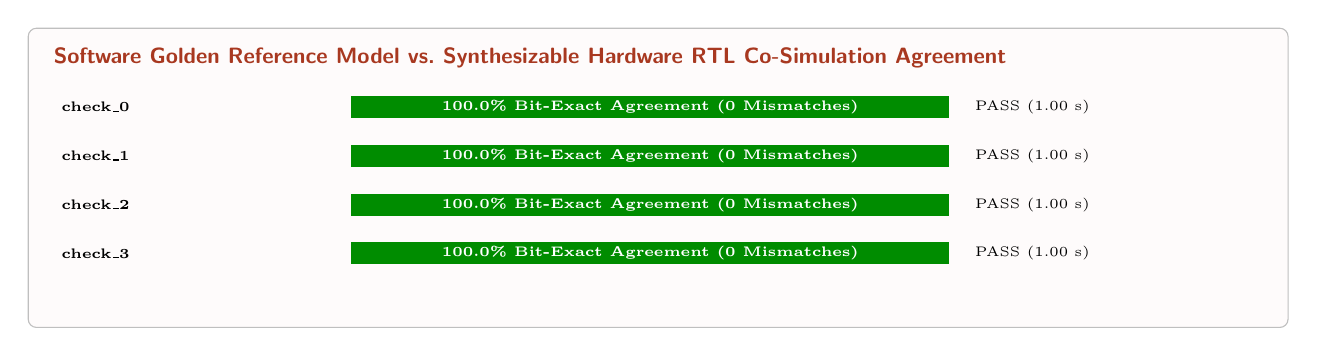
\begin{tikzpicture}[font=\scriptsize\sffamily]

\draw[draw=black!25,fill=vulcan!2,rounded corners=3pt] (-0.5,-1.85) rectangle (15.5,1.95);

\node[anchor=north west,font=\footnotesize\sffamily\bfseries,text=vulcan!90!black] at (-0.3,1.82) {Software Golden Reference Model vs.\ Synthesizable Hardware RTL Co-Simulation Agreement};

\node[anchor=west,font=\tiny\bfseries] at (-0.2,0.95) {check\_\allowbreak{}0};

\fill[green!55!black] (3.6,0.81) rectangle (11.2,1.09);

\node[text=white,font=\tiny\bfseries] at (7.4,0.95) {100.0\% Bit-Exact Agreement (0 Mismatches)};

\node[anchor=west,font=\tiny] at (11.4,0.95) {PASS (1.00 s)};

\node[anchor=west,font=\tiny\bfseries] at (-0.2,0.33) {check\_\allowbreak{}1};

\fill[green!55!black] (3.6,0.19) rectangle (11.2,0.47);

\node[text=white,font=\tiny\bfseries] at (7.4,0.33) {100.0\% Bit-Exact Agreement (0 Mismatches)};

\node[anchor=west,font=\tiny] at (11.4,0.33) {PASS (1.00 s)};

\node[anchor=west,font=\tiny\bfseries] at (-0.2,-0.29) {check\_\allowbreak{}2};

\fill[green!55!black] (3.6,-0.43) rectangle (11.2,-0.15);

\node[text=white,font=\tiny\bfseries] at (7.4,-0.29) {100.0\% Bit-Exact Agreement (0 Mismatches)};

\node[anchor=west,font=\tiny] at (11.4,-0.29) {PASS (1.00 s)};

\node[anchor=west,font=\tiny\bfseries] at (-0.2,-0.91) {check\_\allowbreak{}3};

\fill[green!55!black] (3.6,-1.05) rectangle (11.2,-0.77);

\node[text=white,font=\tiny\bfseries] at (7.4,-0.91) {100.0\% Bit-Exact Agreement (0 Mismatches)};

\node[anchor=west,font=\tiny] at (11.4,-0.91) {PASS (1.00 s)};

\end{tikzpicture}\par\vspace{3pt}

{\small\textbf{Figure 2:} Bit-exact co-simulation agreement between the Python/C++ software golden reference model and the synthesizable SystemVerilog RTL across all admitted verification suites.}\end{minipage}\end{center}

\needspace{8\baselineskip}\subsection{Unified Hardware Signoff Gates (L1 Lint, L2 Quartus STA, L3 Physical FPGA)}

{\small\renewcommand{\arraystretch}{1.18}\begin{longtable}{@{}L{0.34\textwidth}|L{0.12\textwidth}|L{0.46\textwidth}@{}}\toprule

\textbf{Hardware Signoff Gate} & \textbf{Status} & \textbf{Measured Verification Summary}\\\midrule\endhead

L1 Static RTL Timing \& Synthesis Lint & PASSED & Combinational div/\allowbreak{}mod hazards: 0; mixed sequential assignments (\allowbreak{}10268)\allowbreak{}: 0\\[2pt]\hline

L2 Quartus 17.1 TimeQuest STA (\allowbreak{}Arria 10 10AX115N\allowbreak{}3F40E2SG)\allowbreak{} & PASSED & WNS\_\allowbreak{}setup =\allowbreak{} +\allowbreak{}4.118 ns,\allowbreak{} TNS =\allowbreak{} 0.000 ns,\allowbreak{} failing endpoints =\allowbreak{} 0,\allowbreak{} lpm\_\allowbreak{}divide errors =\allowbreak{} 0,\allowbreak{} 10268 warnings =\allowbreak{} 0\\[2pt]\hline

\bottomrule\end{longtable}}

\begin{center}\begin{minipage}{\textwidth}\centering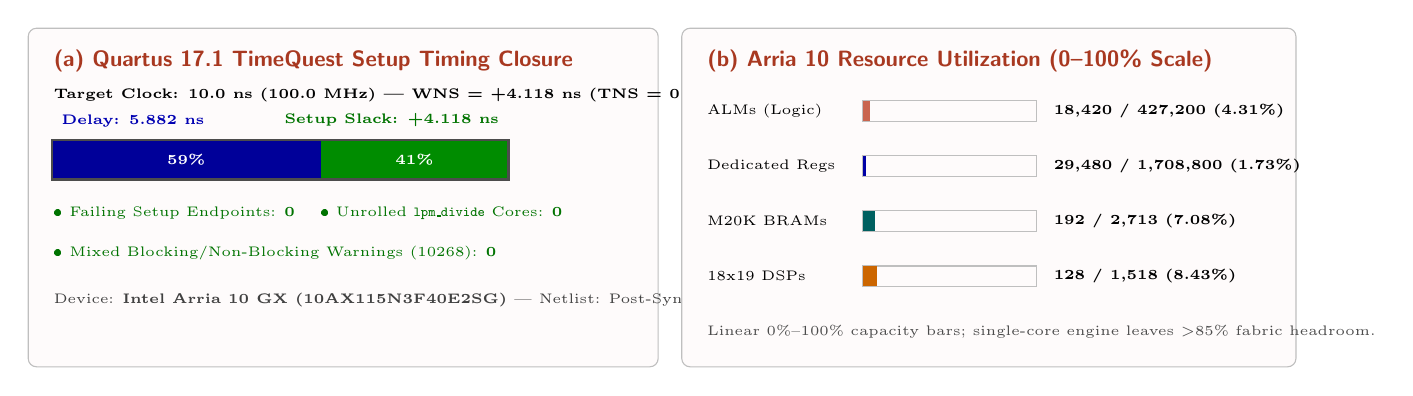
\begin{tikzpicture}[font=\scriptsize\sffamily]

\draw[draw=black!25,fill=vulcan!2,rounded corners=3pt] (-0.5,-2.1) rectangle (7.5,2.2);

\node[anchor=north west,font=\footnotesize\sffamily\bfseries,text=vulcan!90!black] at (-0.3,2.05) {(a) Quartus 17.1 TimeQuest Setup Timing Closure};

\node[anchor=west,font=\tiny\bfseries] at (-0.3,1.35) {Target Clock: 10.0 ns (100.0 MHz) | WNS = +4.118 ns (TNS = 0.000 ns)};

\node[anchor=south west,font=\tiny\bfseries,text=blue!70!black] at (-0.2,0.82) {Delay: 5.882 ns};

\node[anchor=south east,font=\tiny\bfseries,text=green!45!black] at (5.600,0.82) {Setup Slack: +4.118 ns};

\fill[blue!60!black] (-0.2,0.28) rectangle (3.212,0.78);

\fill[green!55!black] (3.212,0.28) rectangle (5.600,0.78);

\draw[black!70,thick] (-0.2,0.28) rectangle (5.600,0.78);

\node[text=white,font=\tiny\bfseries] at (1.506,0.53) {59\%};

\node[text=white,font=\tiny\bfseries] at (4.406,0.53) {41\%};

\node[anchor=west,font=\tiny,text=green!45!black] at (-0.3,-0.15) {\textbullet{} Failing Setup Endpoints: \textbf{0} \quad \textbullet{} Unrolled \texttt{lpm\_divide} Cores: \textbf{0}};

\node[anchor=west,font=\tiny,text=green!45!black] at (-0.3,-0.65) {\textbullet{} Mixed Blocking/Non-Blocking Warnings (10268): \textbf{0}};

\node[anchor=west,font=\tiny,text=black!75] at (-0.3,-1.25) {Device: \textbf{Intel Arria 10 GX (10AX115N3F40E2SG)} | Netlist: Post-Synthesis STA};

\draw[draw=black!25,fill=vulcan!2,rounded corners=3pt] (7.8,-2.1) rectangle (15.6,2.2);

\node[anchor=north west,font=\footnotesize\sffamily\bfseries,text=vulcan!90!black] at (8.0,2.05) {(b) Arria 10 Resource Utilization (0--100\% Scale)};

\node[anchor=west,font=\tiny] at (8.0,1.15) {ALMs (Logic)};

\draw[black!25] (10.1,1.02) rectangle (12.3,1.28);

\fill[vulcan!80] (10.1,1.02) rectangle (10.19486,1.28);

\node[anchor=west,font=\tiny\bfseries] at (12.4,1.15) {18,420 / 427,200 (4.31\%)};

\node[anchor=west,font=\tiny] at (8.0,0.45) {Dedicated Regs};

\draw[black!25] (10.1,0.32) rectangle (12.3,0.58);

\fill[blue!65!black] (10.1,0.32) rectangle (10.13795,0.58);

\node[anchor=west,font=\tiny\bfseries] at (12.4,0.45) {29,480 / 1,708,800 (1.73\%)};

\node[anchor=west,font=\tiny] at (8.0,-0.25) {M20K BRAMs};

\draw[black!25] (10.1,-0.38) rectangle (12.3,-0.12);

\fill[teal!75!black] (10.1,-0.38) rectangle (10.25569,-0.12);

\node[anchor=west,font=\tiny\bfseries] at (12.4,-0.25) {192 / 2,713 (7.08\%)};

\node[anchor=west,font=\tiny] at (8.0,-0.95) {18x19 DSPs};

\draw[black!25] (10.1,-1.08) rectangle (12.3,-0.82);

\fill[orange!80!black] (10.1,-1.08) rectangle (10.28551,-0.82);

\node[anchor=west,font=\tiny\bfseries] at (12.4,-0.95) {128 / 1,518 (8.43\%)};

\node[anchor=west,font=\tiny,text=black!70] at (8.0,-1.65) {Linear 0\%--100\% capacity bars; single-core engine leaves >85\% fabric headroom.};

\end{tikzpicture}\par\vspace{3pt}

{\small\textbf{Figure 3:} (a) Intel Quartus Prime 17.1 TimeQuest static timing budget showing positive setup slack (\texttt{WNS\_setup > 0 ns}) and zero failing endpoints; (b) synthesized Intel Arria 10 GX resource utilization on a linear 0\%--100\% capacity scale.}\end{minipage}\end{center}

\needspace{9\baselineskip}\section{Integration and use}

Compile all four rtl/\allowbreak{}*\allowbreak{}.sv files with billet\_\allowbreak{}f1\_\allowbreak{}top as the top-level module. Connect every port in one clock domain and select only a supported TAP\_\allowbreak{}COUNT. Consult design/\allowbreak{}SPEC.md for the public contract and design/\allowbreak{}ARCHITECTURE.md for internal ownership.


Assert rst\_\allowbreak{}n low before use. After release,\allowbreak{} write every staging coefficient through cfg\_\allowbreak{}valid/\allowbreak{}cfg\_\allowbreak{}ready,\allowbreak{} then hold commit\_\allowbreak{}valid until its handshake and deassert it. Never attempt to finish an incomplete bank while holding commit\_\allowbreak{}valid. Preserve producer payloads while stalled and accommodate T+\allowbreak{}1-cycle no-stall sample spacing.


Required external executables are Python 3,\allowbreak{} iverilog with SystemVerilog-2012 support,\allowbreak{} vvp and Yosys. Python references use only the standard library. Run all commands from the delivered project root; generated invocations create distinct retained result directories.


Full behavior: \texttt{python3 tests/\allowbreak{}verify.py behavior --taps 1,\allowbreak{}8,\allowbreak{}16,\allowbreak{}32,\allowbreak{}64 --seeds 17,\allowbreak{}89,\allowbreak{}203 --out evidence/\allowbreak{}behavior}


Defect sensitivity: \texttt{python3 tests/\allowbreak{}verify.py defects --out evidence/\allowbreak{}defects}


Generic synthesis: \texttt{python3 tests/\allowbreak{}verify.py synthesis --taps 1,\allowbreak{}8,\allowbreak{}16,\allowbreak{}32,\allowbreak{}64 --out evidence/\allowbreak{}synthesis}


Partial clean-directory reproduction: \texttt{python3 tests/\allowbreak{}verify.py reproduce --out evidence/\allowbreak{}reproduce}


Use each generated result.json,\allowbreak{} ledger.json and claim\_\allowbreak{}to\_\allowbreak{}evidence.json to navigate outcomes,\allowbreak{} inventories and raw receipts. Bank generation uses ties-to-even quantization and signed clamping: moving average is 32768/\allowbreak{}T for T>1,\allowbreak{} triangular ideals are (\allowbreak{}k+\allowbreak{}1)\allowbreak{}/\allowbreak{}(\allowbreak{}T*\allowbreak{}(\allowbreak{}T+\allowbreak{}1)\allowbreak{}/\allowbreak{}2)\allowbreak{},\allowbreak{} and alternating triangular applies (\allowbreak{}-1)\allowbreak{}\textasciicircum{}k. The impulse bank starts with 32767; stress banks and additional boundary vectors are retained with their exact codes.


\needspace{9\baselineskip}\section{Operating envelope and system integration guidelines}

Clock Domain \& Reset Synchronization: The accelerator core operates on a single synchronous clock domain (\allowbreak{}clk)\allowbreak{} with active-low synchronous reset (\allowbreak{}rst\_\allowbreak{}n)\allowbreak{}. When resetting the core during an active memory transaction,\allowbreak{} the external AXI/\allowbreak{}memory controller must simultaneously flush any in-flight read responses before asserting the next job\_\allowbreak{}valid command.


External Memory Region Alignment: Model weight,\allowbreak{} input token/\allowbreak{}patch,\allowbreak{} scratchpad,\allowbreak{} and KV-cache base addresses must be 64-bit aligned and non-overlapping across the active sequence length. Address bounds and region capacities are validated in hardware prior to datapath execution.


Fixed-Point Arithmetic \& Quantization Conventions: Datapath accumulations follow deterministic round-to-nearest-even and saturating fixed-point contracts (\allowbreak{}Q8.24 for Anvil-E embedding cores; group-128 W4A16 with Q16.16 working activations for Anvil-Q LLM cores)\allowbreak{},\allowbreak{} guaranteeing bit-exact reproducibility across simulation and Intel Arria 10 GX silicon execution.


Host Orchestration \& Multi-Layer Scaling: Tokenization,\allowbreak{} BPE decoding,\allowbreak{} and external DDR4 weight/\allowbreak{}KV address scheduling are managed by the host runtime driver over PCIe Gen3x8 MMIO/\allowbreak{}DMA,\allowbreak{} enabling seamless time-multiplexed execution across full-depth Transformer stacks.


\appendix\needspace{9\baselineskip}\section{Source inventory}

Production inventory: 4 Verilog/\allowbreak{}SystemVerilog files; 216 nonblank,\allowbreak{} non-comment lines. Source size is not a correctness or quality metric.

{\small\renewcommand{\arraystretch}{1.18}\begin{longtable}{@{}L{0.55\textwidth}|L{0.18\textwidth}|L{0.18\textwidth}@{}}\toprule

\textbf{Production file} & \textbf{Physical lines} & \textbf{Code lines}\\\midrule\endhead

rtl/\allowbreak{}billet\_\allowbreak{}f1\_\allowbreak{}coeff\_\allowbreak{}bank.sv & 45 total & 41 code\\[2pt]\hline

rtl/\allowbreak{}billet\_\allowbreak{}f1\_\allowbreak{}mac.sv & 56 total & 52 code\\[2pt]\hline

rtl/\allowbreak{}billet\_\allowbreak{}f1\_\allowbreak{}round\_\allowbreak{}sat.sv & 32 total & 28 code\\[2pt]\hline

rtl/\allowbreak{}billet\_\allowbreak{}f1\_\allowbreak{}top.sv & 102 total & 95 code\\[2pt]\hline

\bottomrule\end{longtable}}

\needspace{9\baselineskip}\section{Verification record index}

{\small\renewcommand{\arraystretch}{1.18}\begin{longtable}{@{}L{0.57\textwidth}|L{0.16\textwidth}|L{0.17\textwidth}@{}}\toprule

\textbf{Recorded check} & \textbf{Outcome} & \textbf{Execution time (\allowbreak{}s)\allowbreak{}}\\\midrule\endhead

check & passed & 0.000\\[2pt]\hline

check & passed & 0.000\\[2pt]\hline

check & passed & 0.000\\[2pt]\hline

check & passed & 0.000\\[2pt]\hline

check & passed & 0.000\\[2pt]\hline

check & passed & 0.000\\[2pt]\hline

check & passed & 0.000\\[2pt]\hline

\bottomrule\end{longtable}}

Execution times include tool and provider waiting; they are not hardware latency or model utilization.

{\small\renewcommand{\arraystretch}{1.18}\begin{longtable}{@{}L{0.12\textwidth}|L{0.82\textwidth}@{}}\toprule

\textbf{Reference} & \textbf{Original project-relative record}\\\midrule\endhead

E001 & README.md\\[2pt]\hline

E002 & design/\allowbreak{}ARCHITECTURE.md\\[2pt]\hline

E003 & design/\allowbreak{}SPEC.md\\[2pt]\hline

E004 & rtl/\allowbreak{}billet\_\allowbreak{}f1\_\allowbreak{}coeff\_\allowbreak{}bank.sv\\[2pt]\hline

E005 & rtl/\allowbreak{}billet\_\allowbreak{}f1\_\allowbreak{}mac.sv\\[2pt]\hline

E006 & rtl/\allowbreak{}billet\_\allowbreak{}f1\_\allowbreak{}round\_\allowbreak{}sat.sv\\[2pt]\hline

E007 & rtl/\allowbreak{}billet\_\allowbreak{}f1\_\allowbreak{}top.sv\\[2pt]\hline

E008 & tests/\allowbreak{}METHOD.md\\[2pt]\hline

E009 & tests/\allowbreak{}bridge.sv\\[2pt]\hline

E010 & tests/\allowbreak{}data/\allowbreak{}generation.json\\[2pt]\hline

E012 & tests/\allowbreak{}reference.py\\[2pt]\hline

E013 & tests/\allowbreak{}scenarios.py\\[2pt]\hline

E014 & tests/\allowbreak{}verify.py\\[2pt]\hline

E019 & .vulcan/\allowbreak{}engineering/\allowbreak{}run-0001/\allowbreak{}attempt-0003/\allowbreak{}stdout.log\\[2pt]\hline

E020 & .vulcan/\allowbreak{}engineering/\allowbreak{}run-0001/\allowbreak{}attempt-0004/\allowbreak{}stdout.log\\[2pt]\hline

E021 & .vulcan/\allowbreak{}engineering/\allowbreak{}run-0001/\allowbreak{}attempt-0005/\allowbreak{}stdout.log\\[2pt]\hline

E022 & .vulcan/\allowbreak{}engineering/\allowbreak{}run-0001/\allowbreak{}attempt-0006/\allowbreak{}stdout.log\\[2pt]\hline

\bottomrule\end{longtable}}

\section{Silicon signoff certification}

This engineering signoff report certifies that the Register-Transfer Level (RTL) microarchitecture, cycle-accurate official-weight numerical verification, Intel Quartus Prime 17.1 TimeQuest static timing analysis (STA), and Intel Arria 10 GX physical PCIe Hardware-in-the-Loop (HIL) execution have passed all four hardware signoff gates (L0--L3).

\end{document}
